%\usepackage[noend]{algpseudocode}
\chapter{DESAIN}
\label{chapter:design}
Pada bab ini akan dijelaskan mengenai desain algoritma yang digunakan untuk menyelesaikan permasalahan pada Tugas Akhir ini.
\section{Desain Umum Sistem}	
Sistem pertama kali akan menjalankan fungsi MAIN terlebih dahulu. Desain dari fungsi main sendiri dapat dilihat pada gambar \ref{fig:mainfx}. Didalam fungsi main akan di panggil fungsi SOLVE yang digunakan untuk menyelesaikan permasalahan yang diangkat pada tugas akhir ini dan didalam fungsi SOLVE akan terdapat fungsi VALIDITY yang digunakan untuk mengecek kebenaran suatu panjang kunci yang sedang diproses. Secara garis besar fungsi Main.


\begin{figure}[H]
		\centering
		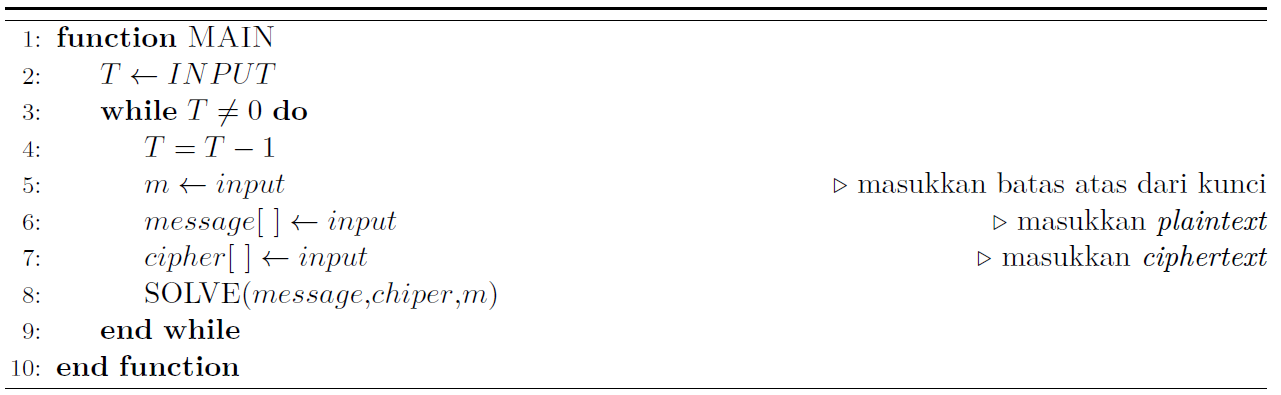
\includegraphics[scale=0.5]{images/bab3/mainfx.png}
		\caption{Gamba Fungsi Main}
		\label{fig:mainfx}
	\end{figure}

\section{Desain Algoritma}
 Pada bagian ini akan dibahas secara rinci mengenai fungsi-fungsi yang digunakan dalam sistem.  
  \subsection{Desain fungsi SOLVE}
  \label{chapter:fxsolve}
  Fungsi ini digunakan untuk menyelesaikan permasalahan yang diangkat pada tugas akhir ini yang didalamnya terdapat tahapan yang telah disebutkan di subbab \ref{chapter:dasar-teori} dan subbab \ref{chapter:solving}, kecuali untuk mengecek kebenaran dari suatu panjang kunci. Gambar mengenai fungsi SOLVE dapat dilihat pada gambar \ref{fig:solvefx}. Mengenai modulo 26 yang terdapat pada gambar digunakan untuk memastikan bahwa sesilih dari \plaintext dan \ciphertext adalah 0 sampai dengan 25, dan ditambah 26 pada gambar dimaksudkan agar silisih antara \plaintext dan \ciphertext selalu bernilai positif.
  
  \begin{figure}[H]
		\centering
		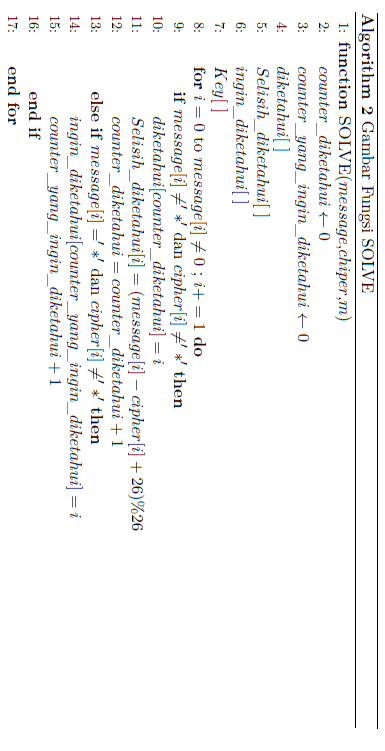
\includegraphics[scale=0.62]{images/bab3/solvefx1.png}
		\caption{Gambar Fungsi SOLVE (1)}
		\label{fig:solvefx}
	\end{figure}
	\begin{figure}[H]
		\centering
		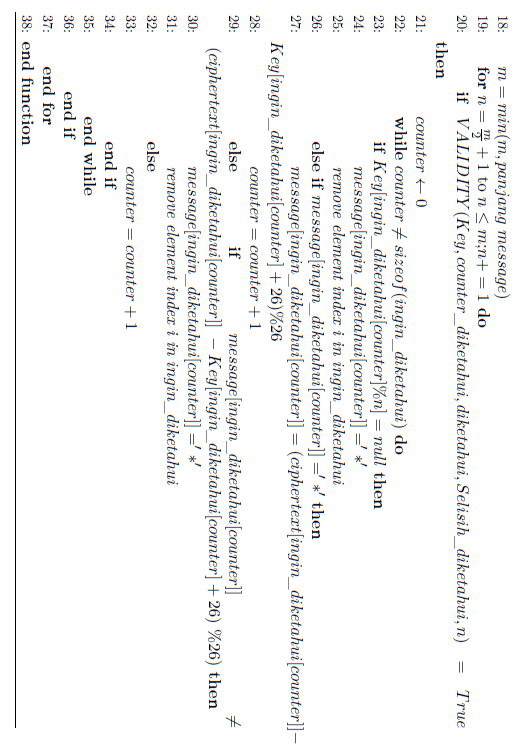
\includegraphics[scale=0.62]{images/bab3/solvefx2.png}
		\caption{Gambar Fungsi SOLVE (2)}
		\label{fig:solvefx}
	\end{figure}
	\subsection{Desain Fungsi VALIDITY}
	Fungsi ini digunakan untuk memvalidasi suatu panjang kunci yang sekarang di cek kebenarannya. Gambar mengenai fungsi VALIDITY dapat dilihar pada gambar \ref{fig:validity}. Penjelasan mengenai fungsi ini terdapat pada subbab \ref{chapter:solving}
	
 \begin{figure}[H]
		\centering
		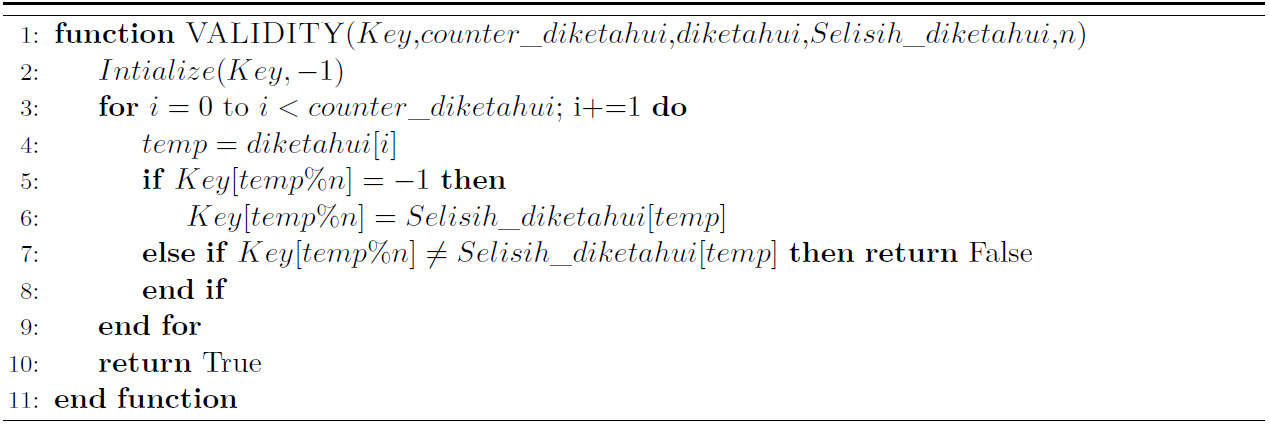
\includegraphics[scale=0.5]{images/bab3/validity.png}
		\caption{Gambar Fungsi VALIDITY}
		\label{fig:validity}
	\end{figure}